% $HeadURL: https://sbgn.svn.sourceforge.net/svnroot/sbgn/ProcessDiagram/tags/L1V1.3Full/sources/perturbing_agent.tex $

\subsection{Glyph: \glyph{Perturbing agent}}
\label{sec:perturbing agent}
 
Biochemical networks can be affected by external influences.  Those
influences can be the effect of well-defined physical perturbing agents, such as a light
pulse or a change in temperature; they can also be more complex and not
well-defined phenomena, for instance the outcome of a biological process, an experimental
setup, or a mutation.  For these situations, SBGN provides the
\glyph{perturbing agent} glyph. It is an EPN, and represents the amount to perturbing agent applied to a process. A \glyph{perturbing agent} is represented by a modified hexagon
having two opposite concave faces, as illustrated in \fig{perturbing agent}.

\begin{figure}[H]
  \centering
  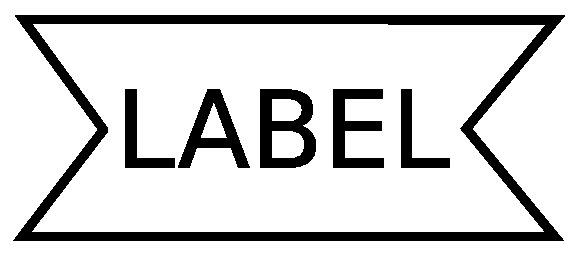
\includegraphics[scale = 0.3]{images/perturbing_agent}
  \caption{The \PD glyph for \glyph{perturbing agent}.}
  \label{fig:perturbing agent}
\end{figure}




% The following is for [X]Emacs users.  Please leave in place.
% Local Variables:
% TeX-master: "../sbgn_PD-level1"
% End:

